\chapter{Versuchergebnisse und Diskussion}
\label{chap:ergebnisse_und_diskussion}

% ----------------------------------------
% Sec: Vergleichsmessung von modifizierten Teilen
% ----------------------------------------
\section{Vergleichsmessung von modifizierten Teilen}
\label{sec:vergleichsmessung_von_difizierten_Teilen}

Vergleich: neue Kugel + neue Scheibe <> neue Kugel + alte Scheibe <> alte Kugel + alte Scheibe <> rechnerische Schmierfilmdicke

% ----------------------------------------
% Fig: Vergleichsmessung von neuer Kugel + neuer Scheibe,
% neuer Kugel + alte Scheibe und theoretische Filmdicke
% ----------------------------------------
\begin{figure}[htb]
    \centering
    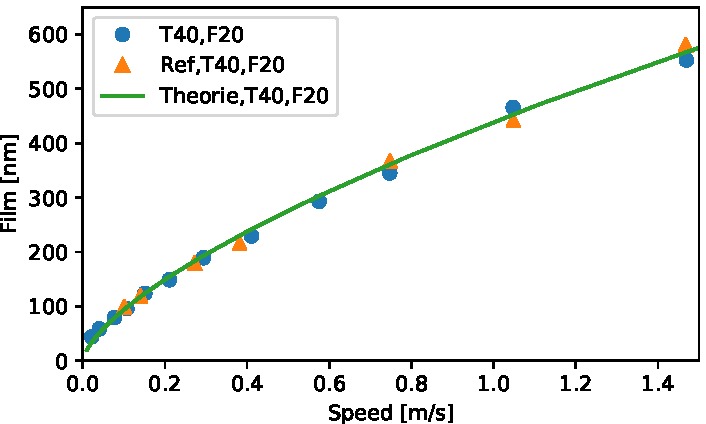
\includegraphics[]{./images/vergleichsmessung_T40_F20_FVA3.pdf}
    \caption{Filmdicke von drei Konfigurationen --- neue Kugel + neue Scheibe (rund); neue Kugel + originale Scheibe (dreieckig); rechnerische Filmdicken (gerade) --- mit dem Öl \textit{FVA 3} bei $T =$ \SI{40}{\degreeCelsius} und $F =$ \SI{20}{\N}}
    \label{fig:vergleichsmessung}
\end{figure}

% ----------------------------------------
% Sec: Messungen mit FVA 3 Öl
% ----------------------------------------
\section{Messungen mit \textit{FVA3}}
\label{sec:messungen_mit_fva3}

\begin{itemize}
    \item Rechnerische Kapazität im EHD-Kontakt.
    \item Einschränkungen von dem mobilen Messsystem von IMKT (geringe Auflösung) -> Benutzung des LCR-Meter
\end{itemize}

